% Section content template for individual Educative lessons
% This file contains the actual content for a specific section
% Generated from Educative API section content

% Section: Requirements of WhatsApp’s Design
% Section ID: 5023065490063360
% Section Slug: requirements-of-whatsapps-design
% Generated: 2025-12-08T14:59:38.946226

\subsection{Requirements}\label{dsaF1YkAhSU5Hievz_XyF}
\\
Our design of the WhatsApp messenger should meet the following requirements.

\subsubsection{Functional requirements}\label{jk-11K5on-rCwYJ7oHmss}

\begin{itemize}
\item
\protect\phantomsection\label{rkGfsEyFJS0bCUZuwiIS-}
\textbf{Conversation}: The system should support one-on-one and group conversations between users.
\item
\protect\phantomsection\label{bKgDaJZz5KOzmYhuzYpey}
\textbf{Acknowledgment}: The system should support message delivery acknowledgment, such as sent, delivered, and read.
\item
\protect\phantomsection\label{rm8NiYdzDCOPFyITfhcj2}
\textbf{Sharing}: The system should support sharing of media files, such as images, videos, and audio.
\item
\protect\phantomsection\label{v_d0RcGLsomCyZlZrNgNn}
\textbf{Chat storage}: The system must support the persistent storage of chat messages when a user is offline until the successful delivery of messages.
\item
\protect\phantomsection\label{c2icROLehfz7igIW7ZU0j}
\textbf{Push notifications}: The system should be able to notify offline users of new messages once their status becomes online.
\end{itemize}
\begin{quote}
\textbf{Note:}~The term ``offline'' typically refers to users not currently connected to the internet. When these users reconnect, the system will automatically send push notifications to alert them of any new messages. On the other hand, the term ``online'' indicates that the user is actively connected to the internet and can receive real-time messages.
\end{quote}
\subsubsection{Non-functional requirements}\label{siPioTRon3FguoSnTc-KQ}

\begin{itemize}
\item
\protect\phantomsection\label{9jmXo8NhQvpl5eu-okW_B}
\textbf{Low latency}: Users should be able to receive messages with low latency.
\item
\protect\phantomsection\label{GsaseMW70ztNsDosbZtC1}
\textbf{Consistency}: Messages should be delivered in the order they were sent. Moreover, users must see the same chat history on all of their devices.
\item
\protect\phantomsection\label{njuEO-74G329-UePDQf6v}
\textbf{Availability}: The system should be highly available. However, the availability can be compromised in the interest of consistency.
\item
\protect\phantomsection\label{AueNOA4_mXhquA1mbysbC}
\textbf{Security}: The system must be secure via end-to-end encryption. The end-to-end encryption ensures that only the two communicating parties can see the content of messages. Nobody in between, not even WhatsApp, should have access.
\item
\protect\phantomsection\label{9ZodKbHNijNpt_4xNfNtZ}
\textbf{Scalability:} The system should be highly scalable to support an ever-increasing number of users and messages per day.
\end{itemize}

\begin{figure}[htbp]
 \centering
 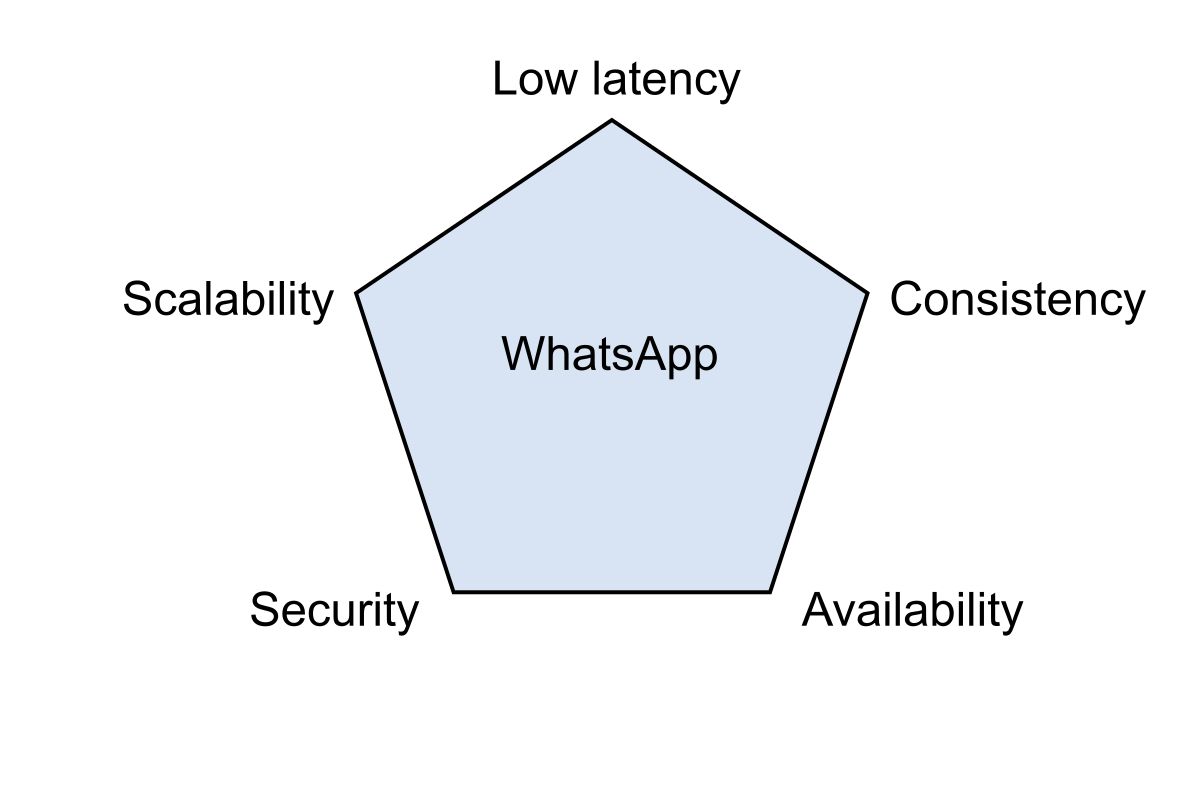
\includegraphics[width=0.25\textwidth]{Images/chapter_36/section_5023065490063360/4787046137462784.png}
 \caption{The non-functional requirements of the WhatsApp system}
\end{figure}

\subsection{Resource estimation}\label{8MCJc79P4JZhMRqqjWIo1}
\\
WhatsApp is the most used messaging application across the globe. According to WhatsApp, it supports more than two billion users around the world who share more than 100 billion messages each day. We need to estimate the storage capacity, bandwidth, and number of servers to support such an enormous number of users and messages.

\subsubsection{Storage estimation}\label{lVQz1i-ag245LGYqSkK1z}
\\
As there are more than 100 billion messages shared per day over WhatsApp, let's estimate the storage capacity based on this figure. Assume that each message takes 100 Bytes on average. Moreover, the WhatsApp servers keep the messages only for 30 days. So , if the user doesn't get connected to the server within these days, the messages will be permanently deleted from the server.
\\
\protect\phantomsection\label{katex_inline_ZX-_ID_LxQVwyyoFEcfTc}{{{\(100\ \text{billion/ day} * 100\ \text{Bytes} = 10\ \text{TB/day}\)}}}
\\
For 30 days, the storage capacity would become the following:
\\
\protect\phantomsection\label{katex_inline_NhvnLODBdQDpB-YV-K60c}{{{\(30 \times10\ \text{TB/day =} 300\ \text{TB/ month}\)}}}
\\
Besides chat messages, we also have media files, which take more than 100 Bytes per message. Moreover , we also have to store users' information and messages' metadata---for example, time stamp, ID, and so on. Along the way, we also need encryption and decryption for secure communication. Therefore, we would also need to store encryption keys and relevant metadata. So
, to be precise, we need more than 300 TB per month, but for the sake of simplicity, let's stick to the number 300 TB per month.

\begin{figure}[htbp]
 \centering
 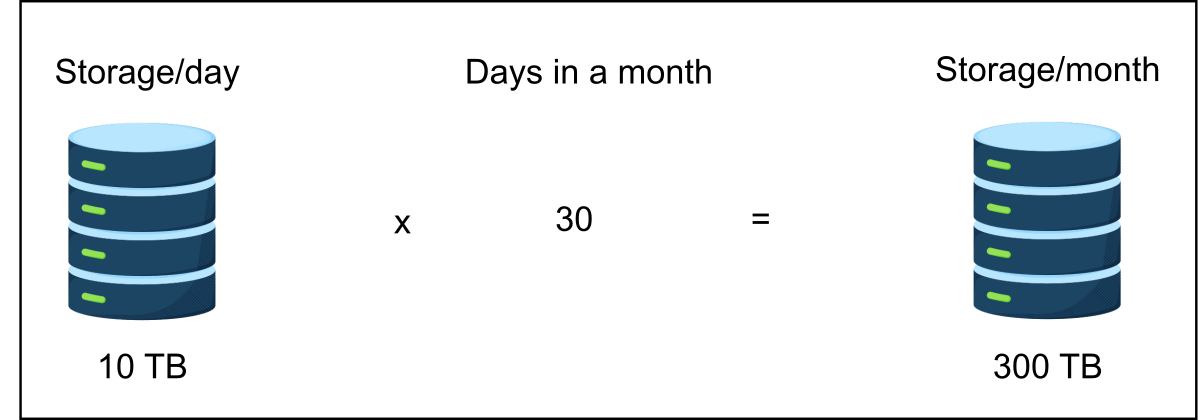
\includegraphics[width=0.5\textwidth]{Images/chapter_36/section_5023065490063360/5686296217780224.png}
 \caption{The total storage required by WhatsApp in a month}
\end{figure}

\subsubsection{Bandwidth estimation}\label{DZXqjLUATg4IlCQGH79xC}
\\
According to the storage capacity estimation, our service will get 10TB of data each day, giving us a bandwidth of 926 Mb/s.
\\
\protect\phantomsection\label{katex_inline_-RejhpW36J1lbXkLLk3At}{{{\(10\ \text{TB}/86400 \text{sec} \approx 926 \text{Mb/s}\)}}}
\begin{quote}
\textbf{Note:} To keep our design simple, we've ignored the media content (images, videos, documents, and so on). So, the number 926 might seem low.
\end{quote}
\\
We also require an equal amount of outgoing bandwidth as the same message from the sender would need to be delivered to the receiver.

\begin{figure}[htbp]
 \centering
 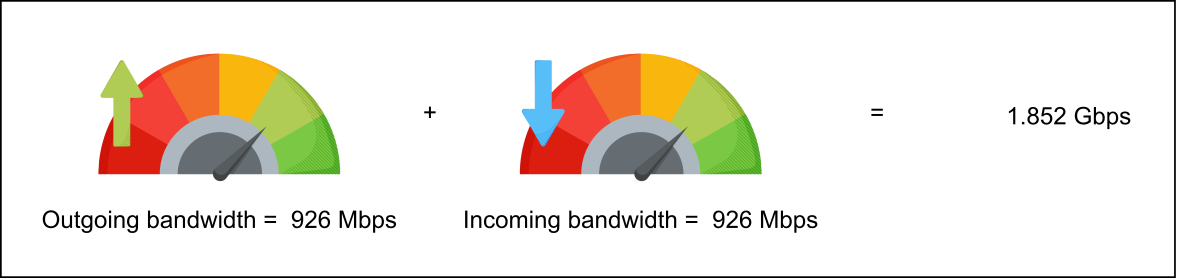
\includegraphics[width=0.5\textwidth]{Images/chapter_36/section_5023065490063360/5804321214431232.png}
 \caption{The total bandwidth required by WhatsApp}
\end{figure}

\textbf{High-level Estimates}

\begin{table}[htbp]
\centering
\small
\adjustbox{max width=\textwidth}{
\begin{tabular}{|p{0.475\textwidth}|p{0.475\textwidth}|}
\hline
\textbf{Type} & \textbf{Estimates} \\
\hline
\hline
Total messages per day & 100 billion \\
\hline
Storage required per day & 10 TB \\
\hline
Storage for 30 days & 300 TB \\
\hline
Incoming data per second & 926 Mb/s \\
\hline
Outgoing data per second & 926 Mb/s \\
\hline
\end{tabular}
}
\caption{High-level Estimates}
\end{table}

\subsubsection{Number of servers estimation}\label{aryDFUfvJxxgAvXJVNUKD}
\\
WhatsApp handles around 10 million connections on a single server, which seems quite high for a server. However, it's possible by extensive performance engineering(For exact details, see the YouTube talk titled C10M Defending The Internet at Scale by Robert Graham.). We 'll need to know all the in-depth details of a system, such as a server's kernel, networking library, infrastructure configuration, and so on.
\begin{quote}
\textbf{Note:} We can often optimize a general-purpose server for special tasks by careful performance engineering of the full software stack.
\end{quote}
\\
Let's move to the estimation of the number of servers:
\\
\protect\phantomsection\label{katex_inline_lMXu3uNDJO-wzN-pix8RI}{{{\(\text{No. of servers} = \frac{\text{Total connections per day}}{\text{No. of connections per server}} = \frac{2 \text{ billion}}{10 \text{ million}} = 200 \text{ servers}<br>\)}}}
\\
So, according to the above estimates, we require 200 chat servers.

\begin{figure}[htbp]
 \centering
 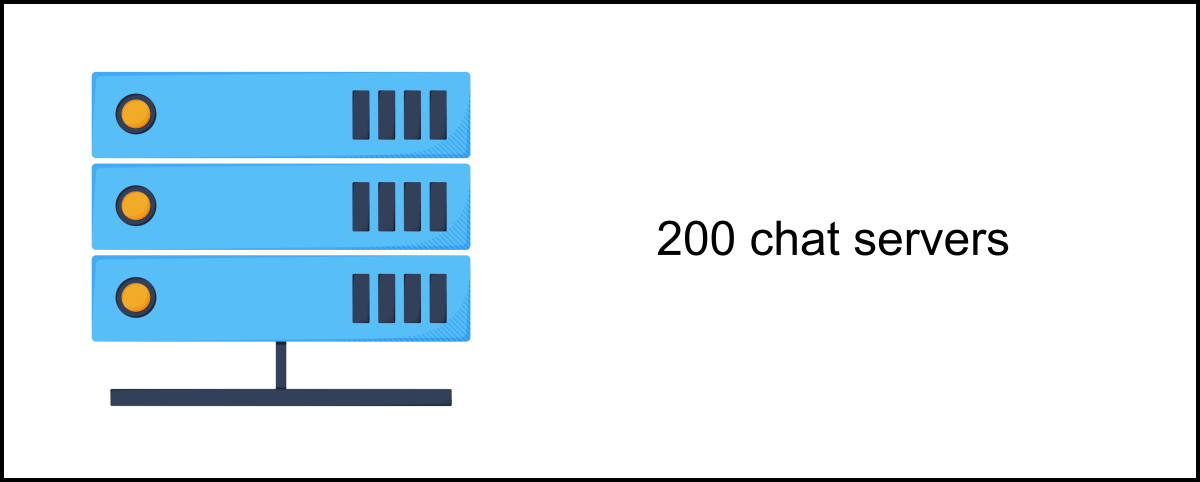
\includegraphics[width=0.5\textwidth]{Images/chapter_36/section_5023065490063360/6080449057521664.png}
 \caption{Number of chat servers required for WhatsApp}
\end{figure}

\subsubsection{Try it out}\label{HTp1tH1EfsifKlL9Kw2iz}
\\
Let's analyze how the number of messages per day affects the storage and bandwidth requirements. For this purpose, we can change values in the following table to compute the estimates:

\subsection{Building blocks we will use}\label{Nke1UStPX05lSExddYrVO}
\\
The design of WhatsApp utilizes the following building blocks that have also been discussed in the initial chapters:

\begin{figure}[htbp]
 \centering
 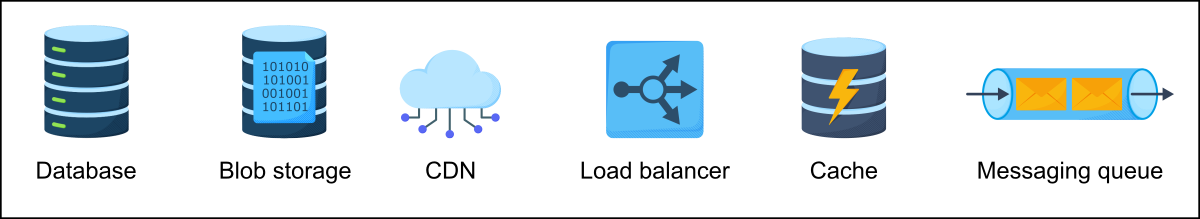
\includegraphics[width=0.5\textwidth]{Images/chapter_36/section_5023065490063360/6601601697841152.png}
 \caption{The building blocks required to design WhatsApp}
\end{figure}

\begin{itemize}
\item
\protect\phantomsection\label{6TQiVBhfLPzx2Syh2nEJO}
\href{https://www.educative.io/courses/grokking-the-system-design-interview/introduction-to-databases}{\textbf{Databases}} are required to store users' and groups' metadata.
\item
\protect\phantomsection\label{_wW10-eYyQSGfR7N1xBF-}
\href{https://www.educative.io/courses/grokking-the-system-design-interview/system-design-a-blob-store}{\textbf{Blob storage}} is used to store multimedia content shared in messages.
\item
\protect\phantomsection\label{u5pceTVZwRfNA-Hd9f0OW}
A \href{https://www.educative.io/courses/grokking-the-system-design-interview/system-design-the-content-delivery-network-cdn}{\textbf{CDN}} is used to effectively deliver multimedia content that's frequently shared.
\item
\protect\phantomsection\label{DTyQNIWMEoEW78sIsG7im}
A \href{https://www.educative.io/courses/grokking-the-system-design-interview/introduction-to-load-balancers}{\textbf{load balancer}} distributes incoming requests among the pool of available servers.
\item
\protect\phantomsection\label{Byjp-Q9lEnt4MLTOMGGZ7}
\href{https://www.educative.io/courses/grokking-the-system-design-interview/system-design-the-distributed-cache}{\textbf{Caches}} are required to keep frequently accessed data used by various services.
\item
\protect\phantomsection\label{9-ZfTEkh46sHvET6wMpXJ}
A \href{https://www.educative.io/courses/grokking-the-system-design-interview/system-design-the-distributed-messaging-queue}{\textbf{messaging queue}} is used to temporarily keep messages in a queue on a database when a user is offline.
\end{itemize}
\\
Evaluate your abilities in designing WhatsApp using the AI widget provided at the end of this lesson. Beyond the mentioned building blocks, additional components contribute to creating a comprehensive design. These include:

\begin{itemize}
\item
Message service
\item
Group message service
\item
Websocket manager
\item
Mnesia database
\item
Redis cluster
\end{itemize}
\\
Provide your solution considering the following details:

\begin{itemize}
\item
Which entity will process the messages of the two users intending to communicate with each other?
\item
How are the group messages handled?
\item
Where are the messages stored when a user is offline?
\item
Where will the media files be kept for frequent access?
\item
What protocol(s) is(are) required to transmit messages with low latency?
\item
How will different services be decoupled?
\end{itemize}

\textbf{Question:}

Design WhatsApp system using the building blocks and components discussed above. 

\textbf{Reference Answer:}

The design of WhatsApp will be composed of the following building blocks and components: a) Data stores: Different types of data require storage in different data stores. We can use structured data such as user and group information data in relational databases such as SQL since WhatsApp stores messages for a short period of time, which it uses the Mnesia database cluster. On the other hand, images and videos shared via WhatsApp are stored in the blob storage.\\
b) Distributed cache: In WhatsApp, each active device is connected to a WebSocket server via WebSocket protocol. The responsibility of WebSocket servers is to provide a port to each online user. The mapping between Websocket servers, ports, and users is stored in the Redis. Redis is an open-source in-memory storage used as a distributed cache. The Redis cluster also caches data from MySQL databases. c) CDN: The content is loaded to CDN if there is a large number of requests for some particular content. The purpose is to efficiently provide the content to the end user. d) Messaging queue: The services are decoupled using the pub-sub, messaging queue, or Kafka. This building block helps us in group messaging. The messaging queue connects the message service and the group message service. The message service is a repository of messages on top of the Mnesia database cluster. The group service keeps all information about users in each group in the system. It has all the information about each group, including user IDs, group IDs, status, group icon, number of users, and so on. This service resides on top of the MySQL database cluster, with multiple secondary replicas distributed geographically. Of course, other than the basic building blocks, there may be other components such as message service, group message service, and WebSocket manager. After describing the components, let's talk about how the functional requirements are met with the help of workflow for the design of WhatsApp. The key functional requirements are: a) The one-on-one and group conversations b) Message delivery acknowledgment such as sent, delivered, and read. c) Support of sharing media files such as images, videos, and audio. d) Persistent storage of chat messages when a user is offline until the successful delivery of messages. e) Notification to offline users once their status becomes online.
\\
Following is the workflow of the WhatsApp design: The communication flow in WhatsApp's detailed design begins with the establishment of communication channels between clients and servers. Each active device connects to a WebSocket server using the WebSocket protocol, with multiple servers catering to the vast user base. The WebSocket manager, residing on a Redis cluster, maintains the mapping between servers, ports, and users. This decentralized approach is necessary to handle the immense scale of billions of users. The
WebSocket server facilitates communication between clients, and the WebSocket manager keeps track of these dynamic connections. When a user initiates a message, the WebSocket server communicates with the WebSocket manager to identify the recipient's WebSocket server. This interaction ensures efficient routing, even in scenarios where the sender and receiver are connected to different servers. Simultaneously , the WebSocket server forwards the message to a message service, acting as an interface to a Mnesia database cluster. This database stores and retrieves messages, serving as a central repository. To ensure secure communication, end-to-end encryption is implemented, providing a robust layer of privacy for users. The intricate interplay between WebSocket servers, WebSocket managers, and message services forms the backbone of WhatsApp's communication infrastructure.
\\
For media files, a specialized asset service handles the process. Files are compressed and encrypted on the sender's device before being sent to the asset service. This service assigns unique IDs to each file and stores them on blob storage. The recipient is informed of the file's presence via the message service, and the file is retrieved using the assigned ID. Group messaging involves components like group message handlers, group message services, and Kafka, facilitating efficient communication within groups. This comprehensive design integrates various components seamlessly, ensuring a scalable and secure communication platform for WhatsApp users. Remember , you can give hints to users on the components to use but avoid giving information on the workflow of the design to meet different functional requirements.

% End of section content